\section{Integration of Forms}

\subsection{Line Integrals}

  \begin{definition}[Orientations, Simple Curves, Closed Curves]
  A path function $p: [a,b]\subset \mathbb{R} \longrightarrow \mathbb{R}^n$ determines a curve in $\mathbb{R}^n$ with endpoints $p(a)$ and $p(b)$. The direction the curve $p$ takes, that is from $p(a)$ to $p(b)$ in $\mathbb{R}^n$ is called the \textit{orientation} of $p$. A path or a curve with a defined orientation is called an \textit{oriented curve}. 

  A \textit{simple curve} $C$ to be the image of an injective piecewise $C^1$ map $c: I \subset \mathbb{R} \longrightarrow \mathbb{R}^3$. Since it is inejctive, it does not intersect itself, and $C$ is piecewise smooth in $\mathbb{R}^n$. If $I = [a,b]$, then $c(a)$ and $c(b)$ are the endpoints of the curve. A simple curve with an orientation is called an \textit{oriented simple curve}. 

  A closed curve $C$ is the image of piecewise $C^1$ map $c: [a,b] \longrightarrow \mathbb{R}^n$ such that $c(a) = c(b)$. That is, the endpoints of $C$ are equal. A \textit{simple closed curve} is a closed curve that is injective over the interval $[a,b)$. Note that a closed curve has two possible orientations. 
  \end{definition}

  If $C$ is an oriented simple curve or an oriented simple closed curve, then we can unambiguously define line integrals along them. 

  \begin{definition}
  Let $h$ be an injective function that takes $[\alpha,\beta] \subset \mathbb{R}$ to the interval $[a, b] \subset \mathbb{R}$. Given an oriented simple path function $p: [a,b]\subset \mathbb{R} \longrightarrow \mathbb{R}^n$, the composition
  \[\rho = p \circ h: [\alpha, \beta] \longrightarrow \mathbb{R}^n\]
  is called a \textit{reparamaterization} of $p$. Note that since $h$ is injective, it takes endpoints to endpoints. If $h$ preserves the direction in which the path travels, that is, if 
  \[(p \circ h)(\alpha) = a \text{ and } (p \circ h)(\beta) = b\]
  then $h$ is \textit{orientation preserving}. If
  \[(p \circ h)(\alpha) = b \text{ and } (p \circ h)(\beta) = a\]
  then $h$ is \textit{orientation reversing}. Note that a path $c$ having the same image as $p$ does not imply that $c$ is a reparamaterization of $p$, since $c$ may not be injective. 
  \begin{center}
      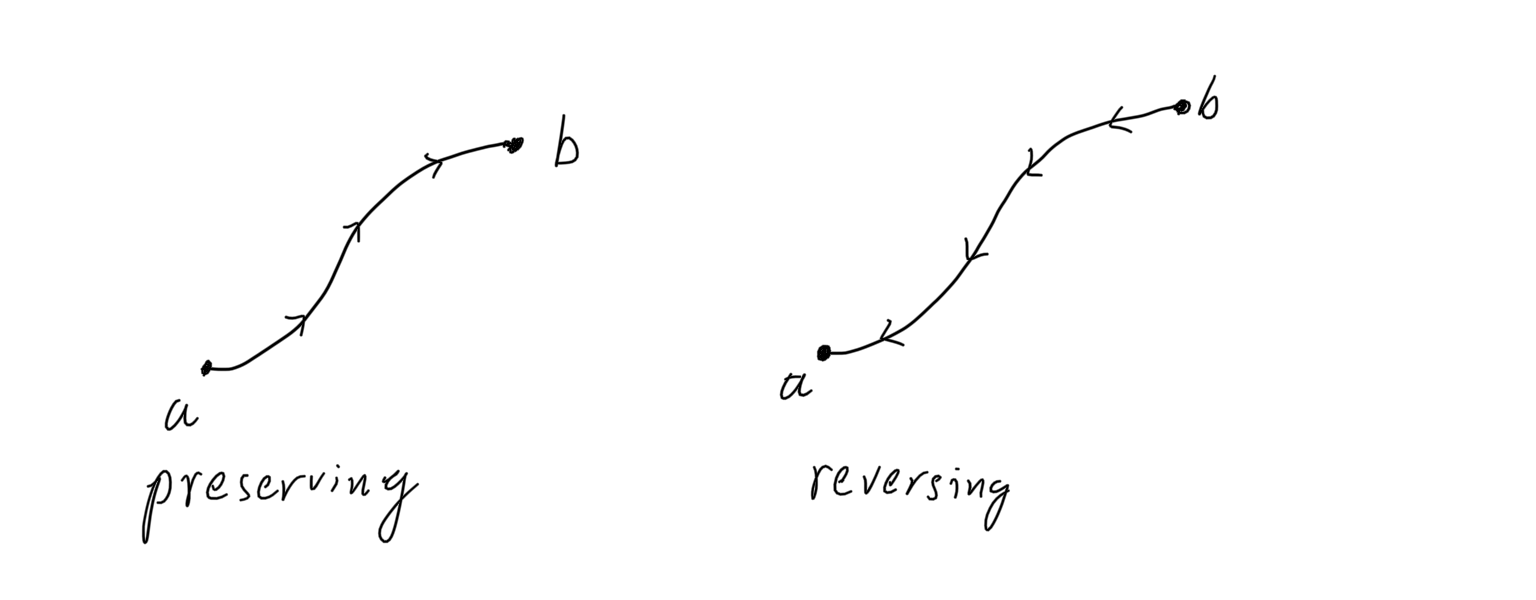
\includegraphics[scale=0.25]{img/Orientation_Preserving_Reversing.PNG}
  \end{center}
  \end{definition}

  \begin{definition}[Scalar Line Integral]
  Let $f: \mathbb{R}^n \longrightarrow \mathbb{R}$, which can be interpreted as a scalar field. Now define a $C^1$ path function 
  \[c: [a,b] \subset \mathbb{R} \longrightarrow \mathbb{R}^n \]
  such that the composition of functions
  \[f \circ c: [a, b] \subset \mathbb{R} \longrightarrow \mathbb{R}^n\]
  is continuous. Then, the \textit{path integral}, or \textit{scalar line integral}, of $f$ along the path $c$. is defined
  \begin{align*}
      \int_c f \;d s & = \int_a^b f\big(c(t)\big) ||c^\prime (t)|| \;d t \\
      & = \int_a^b f\big( x_1 (t), x_2 (t), ..., x_n (t)\big) ||c^\prime (t)|| \; d t
  \end{align*}
  If $c(t)$ is only piece-wise $C^1$, we can define the path integral by breaking $[a,b]$ into pieces over with $f\big( c(t)\big) ||c^\prime (t)||$ is continuous and then summing the integrals over the pieces. 
  That is, 
  \[\int_a^b f\big(c(t)\big) ||c^\prime (t)|| \;d t = \sum_{i = 0}^{n-1} \int_{\alpha_i}^{\alpha_{i+1}} f\big(c(t)\big) ||c^\prime (t)|| \; d t\]
  \end{definition}
  Note that since $f$ is a scalar-valued function, we can interpret a path integral as the sum of infinitesmal segments of the path $c$ having a weight determined by $f$ at each section. 
  If $f$ is a constant function outputting $1$ at every point, then the path integral just outputs the length of the path $c$ in $\mathbb{R}^n$. 
  \[L = \int_a^b f\big( c(t)\big) ||c^\prime (t)|| \; d t = \int_a^b ||c^\prime (t)|| \; d t\]

  \begin{definition}[Vector Line Integral]
  Let $F: \mathbb{R}^n \longrightarrow \mathbb{R}^n$ be a vector field on $\mathbb{R}^n$ that is continuous on the $C^1$ oriented path $c: [a, b] \subset \mathbb{R} \longrightarrow \mathbb{R}^n$. The \textit{line integral} of $F$ along $c$ is defined by the formula 
  \[\int_c F \cdot d s = \int_a^b F\big( c(t)\big) \cdot c^\prime (t) \; d t\]
  where $\cdot$ represents the dot product of $F$ with $c^\prime$ over the interval $[a,b]$. It is also commonly written in differential notation, 
  \[\int_c F \cdot ds = \int_c F \cdot (dx_1, \ldots, d x_n) = \int_c F_1 dx_1 + F_2 dx_2 + \ldots F_n dx_n\]
  \begin{center}
      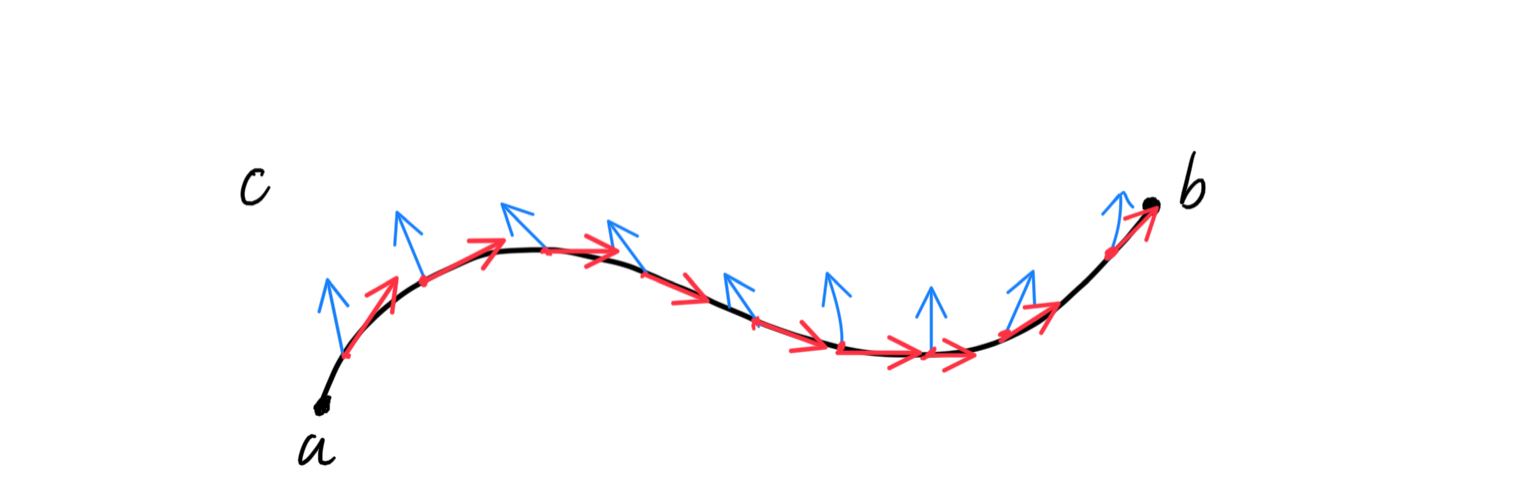
\includegraphics[scale=0.27]{img/Vector_Line_Integral.PNG}
  \end{center}
   Similarly with path integrals, we can also define line integrals as the sum of integrals over piece-wise continuous sections of $c$. That is, given an oriented curve $C$ made up of several oriented component curves $C_i$, $i = 1, 2, ..., k$, we can paramaterize $C$ by paramaterizing the pieces $C_i$'s separately. Thus, we can treat $C = C_1 + ... C_k$ and get
  \[\int_C F \cdot d s = \sum_{i = 1}^k \int_{C_i} F \cdot d s\]
  Note that a vector line integral is a generalization of scalar line integrals, so any results holding for vector line integrals also holds for their scalar counterpart. 
  \end{definition}

  \begin{example}[Work]
  In mechanics, work $W$ is defined as 
  \[W = F \cdot d\]
  where $F$ is force and $d$ is displacement. With this knowledge, the reader can easily see that the work done by vector field $F$ on a particle traveling along a path $c$ from time $a$ to time $b$ can be calculated by the line integral
  \begin{align*}
      W & = \int_a^b F\big( c(t)\big) \cdot c^\prime (t) \; d t \\
      & = \int_c F_1 dx + F_2 dy + F_3 dz
  \end{align*}
  \end{example}

  \begin{theorem}[Invariance of Path Paramaterizations on Vector Line Integrals]
  Let $F$ be a vector field and $f$ be a scalar field, both continuous on the $C^1$ path function $p: [a,b] \longrightarrow \mathbb{R}^n$ and let $q: [\alpha, \beta] \longrightarrow \mathbb{R}^n$ be a reparamaterization of $p$. Then, 
  \begin{align*}
      q \text{ is orientation preserving} & \implies \int_p F \cdot d s = \int_q F \cdot d s \\
      q \text{ is orientation reversing} & \implies \int_p F \cdot d s = - \int_q F \cdot d s
  \end{align*}
  \end{theorem}

\subsection{Conservative Vector Fields}

  We now introduce a fundamental theorem about line integrals over gradient fields. Recall the fundamental theorem of calculus and it's equivalent form. 

  \begin{theorem}[Fundamental Theorem of Single Variable Calculus]
  Let function $\nabla g: \mathbb{R} \longrightarrow \mathbb{R}$ be the gradient of the single variable $C^1$ function $g: \mathbb{R} \longrightarrow \mathbb{R}$; that is, $\nabla g$ is a conservative vector field on $\mathbb{R}$. Then, 
  \[\int_a^b \nabla g (x) \,dx = g(b) - g(a)\]
  Note that in the single variable case, 
  \[\frac{d}{dx} g(x) = \nabla g(x)\]
  This means that the value of the integral of $\nabla g$ only depends on the value of $g$ at the endpoints of the interval $[a,b]$. 
  \end{theorem}

  We can extend this to line integrals for functions mapping $\mathbb{R}^n$ to $\mathbb{R}$. 

  \begin{theorem}[Invariance of Line Integrals in Conservative Vector Fields]
  Given that $F: \mathbb{R}^n \longrightarrow \mathbb{R}^n$ is a $C^1$ conservative vector field with $\nabla f = F$ for $C^2$ function $f: \mathbb{R}^n \longrightarrow \mathbb{R}$ and path function $p: [a,b] \longrightarrow \mathbb{R}^n$ is a piecewise $C^1$ path, then 
  \[\int_p F \cdot d s = \int_p \nabla f \cdot d s = f\big(p(b)\big) - f\big(p(a)\big)\]
  That is, the line integral of any path in a conservative vector field is dependent on the value of $f$ at the endpoints $p(a)$ and $p(b)$. 
  \begin{center}
      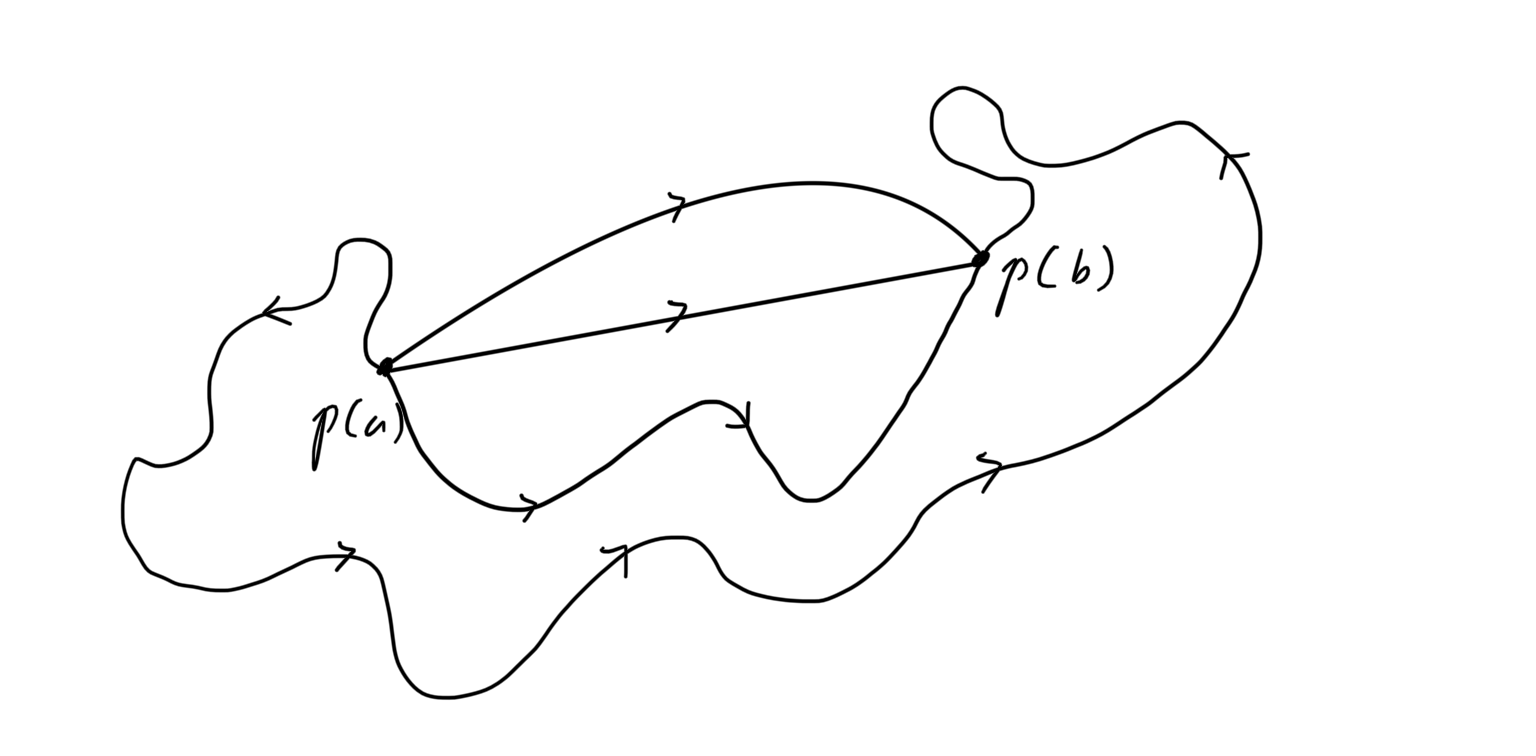
\includegraphics[scale=0.2]{img/Line_Integral_Independence_of_path.PNG}
  \end{center}
  \end{theorem}

  In physics, calculating the work done by a force represented by a vector field requires us to know the path that it travels through. 
  \[W = \int_p F \cdot ds\]
  However, in many cases $F$ is assumed to be conservative, so it is only necessary that we find the displacement of the particle from its endpoints, resulting in the simplification of the formula.  
  \[W = \int_p \nabla f \cdot ds = f\big( p(b)\big) - f \big(p(a)\big)\]

  \begin{corollary}[Equivalent Conditions for Vector Field to be Conservative]
  The following conditions are equivalent: 
  \begin{enumerate}
      \item $F: \mathbb{R}^n \longrightarrow \mathbb{R}^n$ is a conservative vector field. 
      \item The line integral of $F: \mathbb{R}^n \longrightarrow \mathbb{R}^n$ in curve $C$ is path independent; that is, if $C_1$ and $C_2$ are two paramaterizations of $C$, 
      \[\int_{C_1} F \cdot ds = \int_{C_2} F \cdot ds\]
      \item Given that $C$ is a closed loop, the line integral of $F: \mathbb{R}^n \longrightarrow \mathbb{R}^n$ across $C$ is $0$. 
      \[\oint_C F \cdot ds = 0\]
      \item The curl of $F: \mathbb{R}^3 \longrightarrow \mathbb{R}^3$ vanishes
      \[\curl{F} = \nabla \times F = \begin{pmatrix}
      \frac{\partial F}{\partial x} \\\frac{\partial F}{\partial y} \\\frac{\partial F}{\partial z} 
      \end{pmatrix} \times \begin{pmatrix}
      F_1\\F_2\\F_3
      \end{pmatrix}= 0\]
      \item The following partial derivatives of $F: \mathbb{R}^2 \longrightarrow \mathbb{R}^2$ are equal
      \[\frac{\partial F_1}{\partial y} = \frac{\partial F_2}{\partial x}\]
  \end{enumerate}
  \end{corollary}

  We can develop a bit of intuition to determine whether a vector field is conservative or not. If vector field $F$ is conservative, then there exists a smooth scalar field $f$ such that $\nabla f = F$. For each latitude and longitude on a certain map, we can give it an altitude as a function of those coordinates (picture a map with a bunch of hills and valleys). The gradient and thus the vector field is all the vectors that point in the direction of highest ascent. he vector field is all the vectors that point in the direction of highest ascent. Extending the metaphor the path integral is like starting on at a point and climbing the hills and valleys, creating work as you go up a hill (proportional to the steepness and thus the dot product of your motion vector with the gradient vector field in the path integral) and decreasing the work you put in by going down a hill. Since the path is closed, it is like you are going up and down the same amount overall, so the path integral is zero. Following this analogy, the vector field determined by this function (marked as arrows in the $x, y$ plane) is conservative. 
  \begin{center}
      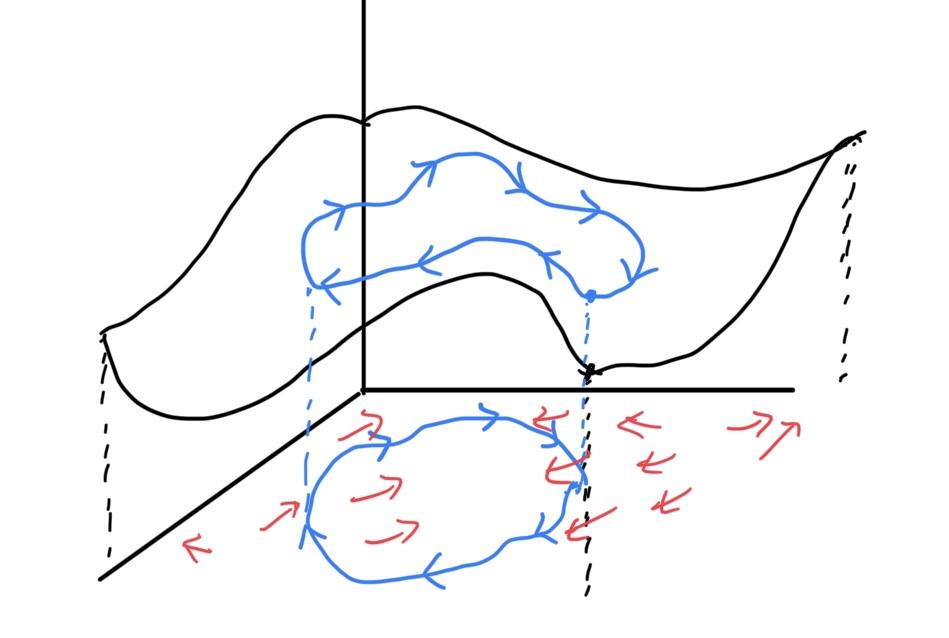
\includegraphics[scale=0.28]{img/Conservative_Vector_Field.jpg}
  \end{center}
  If we can construct a closed loop around $F$ where the line integral is nonzero, then it means that we have ended up at a "higher" or "lower" (altitude) at the same point. This means that rather than being a certain landscape, there exist different "levels" of values at one point, like a spiraling staircase. For example, look at the solenoidal vector field below, where we can construct a closed loop (a circle going around the origin counterclockwise). There is no "surface" that can be defined such that it contains the solenoid. 
  \begin{center}
      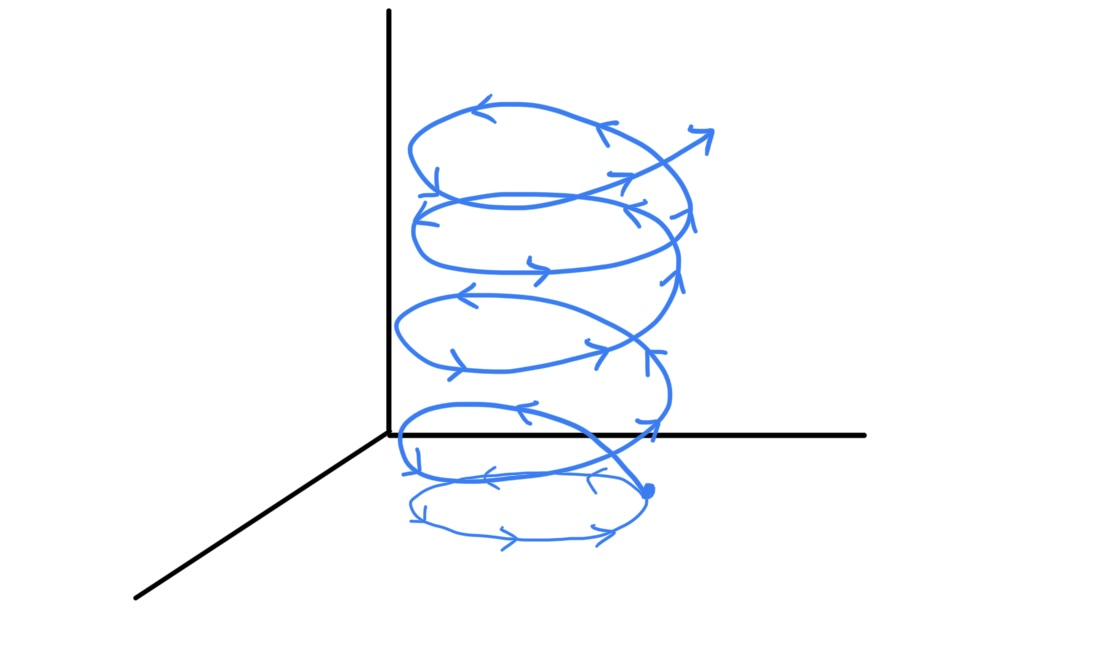
\includegraphics[scale=0.28]{img/Solenoid_nonconservative.jpg}
  \end{center}
  Clearly, as a particle travels through the vector field along the path, it does positive work while it has zero displacement, and clearly, there exists no function that can output both these values as determined by vector field $F$. 

  \begin{theorem}[Helmholtz Decomposition]
  Let $F: \mathbb{R}^3 \longrightarrow \mathbb{R}^3$ be a $C^2$ vector field. Then, $F$ can be decomposed into a curl-free component and a divergence-free component. That is, there exists vector fields $A$ and $\Phi$
  \[F = - \nabla \cdot \Phi + \nabla \times A\]
  \end{theorem}

  \subsubsection{Curvature}
  \begin{definition}[Curvature at a Point]
  Let $c: [a, b] \longrightarrow C \subset \mathbb{R}^3$ be a unit-speed paramaterization of $C$, meaning that $||c^\prime (t)|| = 1$ for all $t \in [a,b]$, and let $p = c(t_0)$ be a point in $C$. The \textit{curvature} $\kappa(p)$ at $p$ is a mapping defined
  \[\kappa: C \longrightarrow \mathbb{R}, \;\; \kappa(p) \equiv ||c^{\prime \prime} (t_0)||\]
  Notice that since we require a unit speed paramaterization of $C$, we do not need to worry about how a given curve is paramaterized. 
  \end{definition}

  Since the curvature is defined pointwise for each point in curve $C$, we can integrate over all the curvatures in $C$ to define the total curvature. 

  \begin{definition}[Total Curvature]
  The \textit{total curvature} of a curve $c: [a,b] \longrightarrow C \subset \mathbb{R}^3$ is the scalar line integral 
  \[\int_C \kappa \, ds\]
  \end{definition}

  We now present an important theorem in differential geometry. 
  \begin{theorem}[Fary-Milnor Theorem]
  Given a unit speed paramaterization $c: [a,b] \longrightarrow C \subset \mathbb{R}^3$, if $C$ is closed (that is, $c(a)=c(b)$), then 
  \[\oint_C \kappa\, ds \geq 2 \pi\]
  and equals $2\pi$ only when $C$ is a circle. Furthermore, if $C$ is a closed space curve with 
  \[\oint_C \kappa\, ds \leq 4\pi\]
  then $C$ is "unknotted." That is, $C$ can be continuously deformed without every intersecting itself into a planar circle. Therefore, for knotted curves $C$, we have
  \[\oint_C \kappa \, ds > 4\pi\]
  \end{theorem}

\subsection{Surface Integrals}

  Surface integrals are the $2$-dimensional analogue, or the double integral version, of line integrals. It is the integration of surfaces. 

  \subsubsection{2-Dimensional Paramaterizations of Surfaces}
  Just like how we create path functions using a paramaterization function $p: [a, b] \subset \mathbb{R} \longrightarrow \mathbb{R}^n$, we can parameterize surfaces by defining a function 
  \[\varphi: D \subset \mathbb{R}^2 \longrightarrow \mathbb{R}^n, \;\;\; \varphi (u, v) \equiv \begin{pmatrix} x_1 (u, v) \\ \vdots \\ x_n (u, v) \end{pmatrix}\]
  The surface 
  \[S = \varphi(D)\]
  corresponding to the function $\varphi$ is its image. If $\varphi$ is differentiable or is of class $C^1$, then we call $S$ a \textit{differentiable} or $C^1$ surface, respectively. 

  For those that are familiar with differential geometry, this makes every paramaterized surface a 2-manifold induced by the single homeormophism $\varphi$. In fact, it is more than just locally homeomorphic; it is \textit{globally} homeomorphic. 


  \begin{definition}[Tangent Vectors of Surfaces Embedded in $\mathbb{R}^3$]
  Given surface paramaterization 
  \[\varphi: \mathbb{R}^2 \longrightarrow \mathbb{R}^3, \;\;\; \varphi(u, v) \equiv \begin{pmatrix}
  x (u, v) \\ y(u, v) \\ z(u, v) 
  \end{pmatrix}\]
  it is visually clear that there can be up to two linearly independent tangent vectors at a point on the surface $S$. We can calculate these two vectors by embedding two nonparallel paths in $D \subset \mathbb{R}^2$ and taking the derivative with respect to a point traveling through these paths, which would give us a tangent vector on $S$. To keep things simple, we take the partial derivatives with respect to $u$ and $v$. 
  \begin{center}
      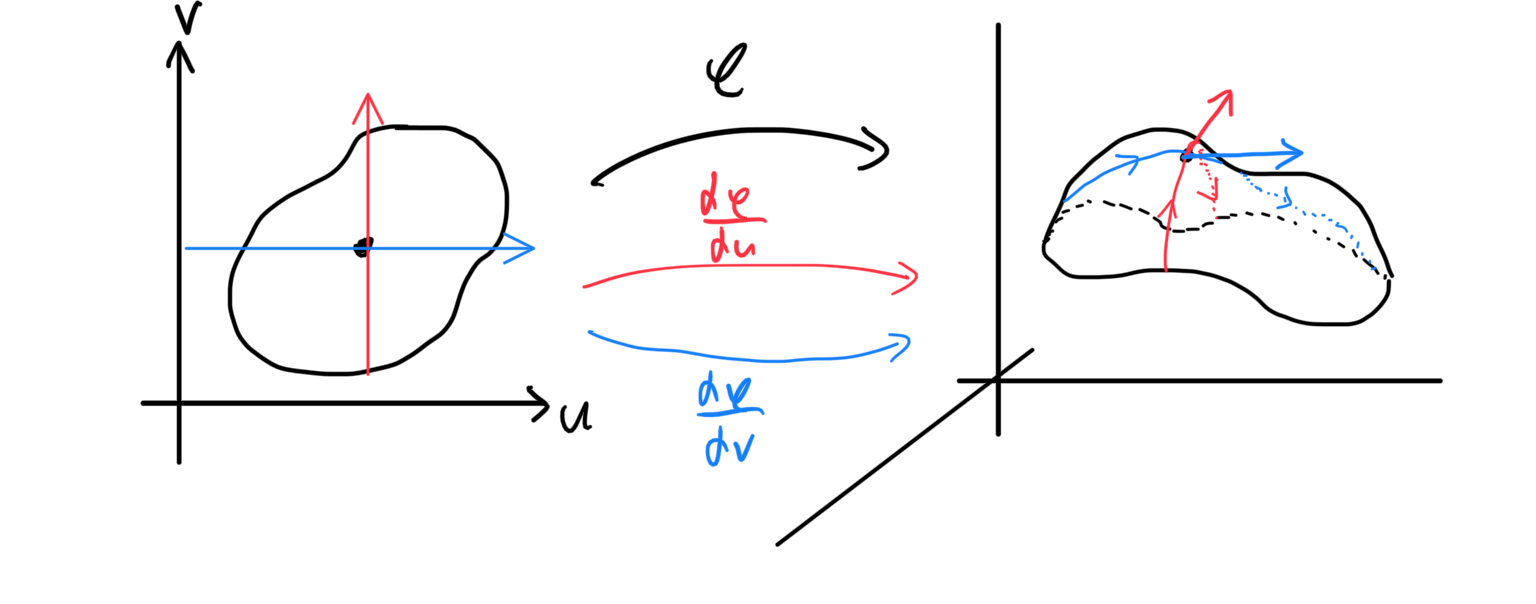
\includegraphics[scale=0.28]{img/Partial_Derivatives_with_respect_to_U_V.PNG}
  \end{center}
  Clearly, these paths are functions 
  \begin{align*}
      \frac{\partial \varphi}{\partial u} \equiv \begin{pmatrix}
       \frac{\partial x}{\partial u} \\ \frac{\partial y}{\partial u} \\ \frac{\partial z}{\partial u}
      \end{pmatrix} : \mathbb{R}^2 \longrightarrow \mathbb{R}^3\\
      \frac{\partial \varphi}{\partial v} \equiv \begin{pmatrix}
       \frac{\partial x}{\partial v} \\ \frac{\partial y}{\partial v} \\ \frac{\partial z}{\partial v}
      \end{pmatrix} : \mathbb{R}^2 \longrightarrow \mathbb{R}^3
  \end{align*}
  where 
  \[\frac{\partial \varphi}{\partial u} (u_0 ,v_0), \; \frac{\partial \varphi}{\partial v} (u_0, v_0)\]
  represent two vectors in $\mathbb{R}^3$ that are tangent to $S$ at the point $\varphi(u_0, v_0) \in \mathbb{R}^3$. 
  \end{definition}

  We must make sure that the surface $S$ is smooth in the sense that (informally) there aren't any wrinkles, points, folds, or self-intersections in such a way that the tangent plane to the surface is not well-defined. 

  \begin{definition}[Regular Surfaces]
  To formalize this concept, we say that $S$ is \textit{regular}, or \textit{smooth}, at point $(u_0, v_0)$ if
  \[\frac{\partial \varphi}{\partial u} \times \frac{\partial \varphi}{\partial v} \neq 0\]
  where $\times$ is the Euclidean cross product. That is, if the vector that is orthogonal to the two tangent vectors is well defined at a point, the surface is said to be smooth at that point. Note that $\frac{\partial \varphi}{\partial u}$ is parallel to $\frac{\partial \varphi}{\partial v}$ if and only if their cross product is $0$. 
  \begin{center}
      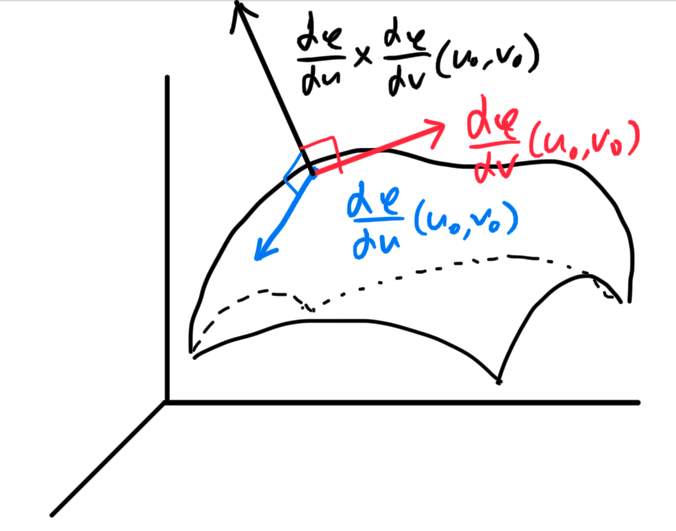
\includegraphics[scale=0.3]{img/Cross_Product_Regular_Surfaces.PNG}
  \end{center}
  It is quite clear that $(\frac{\partial \varphi}{\partial u} \times \frac{\partial \varphi}{\partial v})(u_0, v_0) \neq 0 \implies \frac{\partial \varphi}{\partial u}$ and $\frac{\partial \varphi}{\partial v}$ are linearly independent. This means that an entire span of tangent vectors, i.e. a tangent plane, of the surface $S$ at $\varphi(u_0, v_0)$ exists. 
  $S$ is said to be \textit{regular} if it is regular at all points $\varphi(u_0, v_0) \in S$. 
  \end{definition}

  In fact, the tangent plane at $\varphi(u_0, v_0)$ is the set of points 
  \[\{\varphi(u_0, v_0) + \frac{\partial \varphi}{\partial u} (u_0, v_0) c_1 + \frac{\partial \varphi}{\partial v} (u_0, v_0) c_2 \; | \; c_1, c_2 \in \mathbb{R} \}\]
  which is precisely the affine tangent plane spanned by $T_u$ and $T_v$. Note also that the vector $T_u \times T_v$, if nonzero, is normal to this plane, which leads to this equivalent definition. 

  \begin{definition}[Tangent Planes of Surfaces]
  Given a paramaterized surface $\varphi: D \subset \mathbb{R}^2 \longrightarrow \mathbb{R}^3$ that is regular at $\varphi(u_0, v_0)$, the tangent plane of the surface $S$ at $\varphi(u_0, v_0) = (x_0, y_0, z_0)$ is defined
  \[\{(x, y, z) \in \mathbb{R}^3 \;|\; (x-x_0, y-y_0, z-z_0) \cdot n = 0\}\]
  where $n = (\frac{\partial \varphi}{\partial u} \times \frac{\partial \varphi}{\partial v})(u_0, v_0)$. 
  \end{definition}

  We finally construct the concept of signed areas before defining surface integration. 
  We have all the tools we need to calculate surface areas, but remember that integration also covers the concept of \textit{signed areas}, which could be negative. In order to define this, we define the concept of orientation on surfaces. 

  \subsubsection{Orientation of Surfaces}

  \begin{definition}[Oriented Surfaces]
  An \textit{oriented surface} is a two-sided surface with one side specified as the \textit{outside/positive} side and the other side as the \textit{inside/negative} side. Note that an oriented surface is not guaranteed to have two sides (e.g. a Mobius strip). To ensure that there exist two sides, $S$ must be regular. 

  Surprisingly, a paramaterization does not have an intrinsic orientation. Rather, we determine the orientation ourselves by choosing a unit vector that generally points towards the outside of the surface $S$. Again, this choice is arbitrary, but it is customary to choose a vector that generally points "out." Either way, the orientation (unit) vector at every point $\varphi(u, v) \in S$, denoted as $n$, is 
  \[n\big(\varphi(u, v)\big) = \pm \frac{\frac{\partial \varphi}{\partial u} \times \frac{\partial \varphi}{\partial v}}{\big|\big|\frac{\partial \varphi}{\partial u} \times \frac{\partial \varphi}{\partial v}\big|\big|}\]
  which can be visually calculated using the right hand rule. 
  \begin{center}
      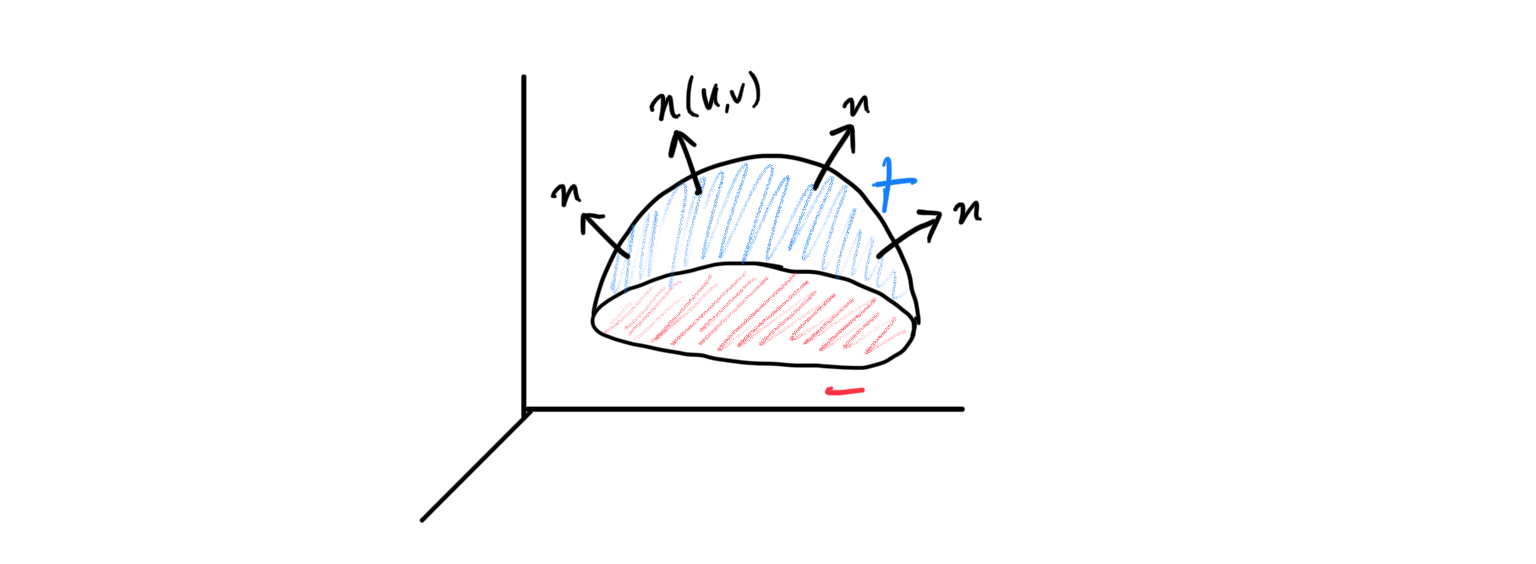
\includegraphics[scale=0.23]{img/Orientation_Unit_Vector.PNG}
  \end{center}
  \end{definition}

  \begin{definition}[Orientation Preserving, Reversing Paramaterizations]
  Given an oriented surface $S$ with its positive side determined by the direction of unit vector $n\big( \varphi(u,v)\big)$, the paramaterization $\varphi$ is said to be \textit{orientation preserving} if 
  \[n \big( \varphi(u, v)\big) = \frac{\frac{\partial \varphi}{\partial u} \times \frac{\partial \varphi}{\partial v}}{\big|\big|\frac{\partial \varphi}{\partial u} \times \frac{\partial \varphi}{\partial v}\big|\big|}\]
  and \textit{orientation reversing} if
  \[n \big( \varphi(u, v)\big) = - \frac{\frac{\partial \varphi}{\partial u} \times \frac{\partial \varphi}{\partial v}}{\big|\big|\frac{\partial \varphi}{\partial u} \times \frac{\partial \varphi}{\partial v}\big|\big|}\]
  \end{definition}

  So, to find whether a paramaterization is orientation preserving or reversing, it suffices to find the cross product $T_u \times T_v$ and see if it points in the same direction of the normal vector $n$ (which should have already been determined when deciding the orientation of $S$). 

  Given a paramaterization $\varphi$ and an un-oriented surface $S$, we can also just construct $\varphi$ to be orientation-preserving (or reversing) by \textit{defining} the normal vector $n$ to be 
  \[n\big( \varphi(u, v)\big) = \frac{\frac{\partial \varphi}{\partial u} \times \frac{\partial \varphi}{\partial v}}{\big|\big|\frac{\partial \varphi}{\partial u} \times \frac{\partial \varphi}{\partial v}\big|\big|} \;\; \bigg( \text{or } n\big( \varphi(u, v)\big) = - \frac{\frac{\partial \varphi}{\partial u} \times \frac{\partial \varphi}{\partial v}}{\big|\big|\frac{\partial \varphi}{\partial u} \times \frac{\partial \varphi}{\partial v}\big|\big|} \bigg)\]
  So rather than finding out whether a paramaterization $\varphi$ is orientation preserving or reversing by comparing $T_u \times T_v$ with $n$, we have defined $n$ in a way such that $\varphi$ must be orientation preserving (or reversing). We can utilize these tools of paramaterization to now define the surface integral. 

  \subsubsection{Scalar, Vector Surface Integrals}

  A physical interpretation of a scalar surface integral is the weighted surface area of a certain surface. 

  \begin{definition}[Scalar Surface Integrals]
  Let $f: \mathbb{R}^3 \longrightarrow \mathbb{R}$ be a $C^1$ scalar field defined on a paramaterized surface $S \subset \mathbb{R}^3$ with paramaterization $\varphi: D \subset \mathbb{R}^2 \longrightarrow \mathbb{R}^3$. That is, $\varphi(D) = S$. We define the integral $f$ over $S$ to be
  \begin{align*}
      \iint_S f \; dS & = \iint_S f(x, y, z) \; dS \\
      & = \iint_D f\big( \varphi(u, v)\big) \bigg|\bigg|\frac{\partial \varphi}{\partial u} \times \frac{\partial \varphi}{\partial v}\bigg|\bigg| \; du \,dv
  \end{align*}
  Note that this will require us to transform $f$, a function of $x, y, z$, into the function $f \circ \varphi$ of $u, v$. Additionally, if the paramaterization of the surface $S$ is not defined, then it one must be constructed. It is also clear that if $S$ is a union of surfaces $S_i$, then its surface integral is the sum of the surface integrals of the $S_i$'s. 
  \end{definition}

  Letting the scalar field $f$ be the constant field equal to $1$, the scalar surface integral measures the surface area of $S$. 
  \[A(S) = \iint_S \; dS = \iint_D \Big|\Big|\frac{\partial \varphi}{\partial u} \times \frac{\partial \varphi}{\partial v}\Big|\Big| \; du\, dv\]
  It is easy to see that the orientation of the paramaterization $\varphi$ does not affect scalar surface integrals, since the sign of the orientation gets nullified by the absolute value sign over $||\frac{\partial \varphi}{\partial u} \times \frac{\partial \varphi}{\partial v}||$. 

  Its physical interpretation is to measure the rate at which a fluid (determined by a vector field $F$) is crossing a given surface $S$. It also has many applications in electromagnetism. 

  \begin{definition}[Vector Surface Integrals]
  Let $F$ be a vector field defined on surface $S$, the image of a paramaterized surface $\varphi$. The \textit{surface integral} of $F$ over $S$ is defined below, which is equivalent to summing up the dot product of the vector field and the normal vector to the surface. 
  \begin{center}
      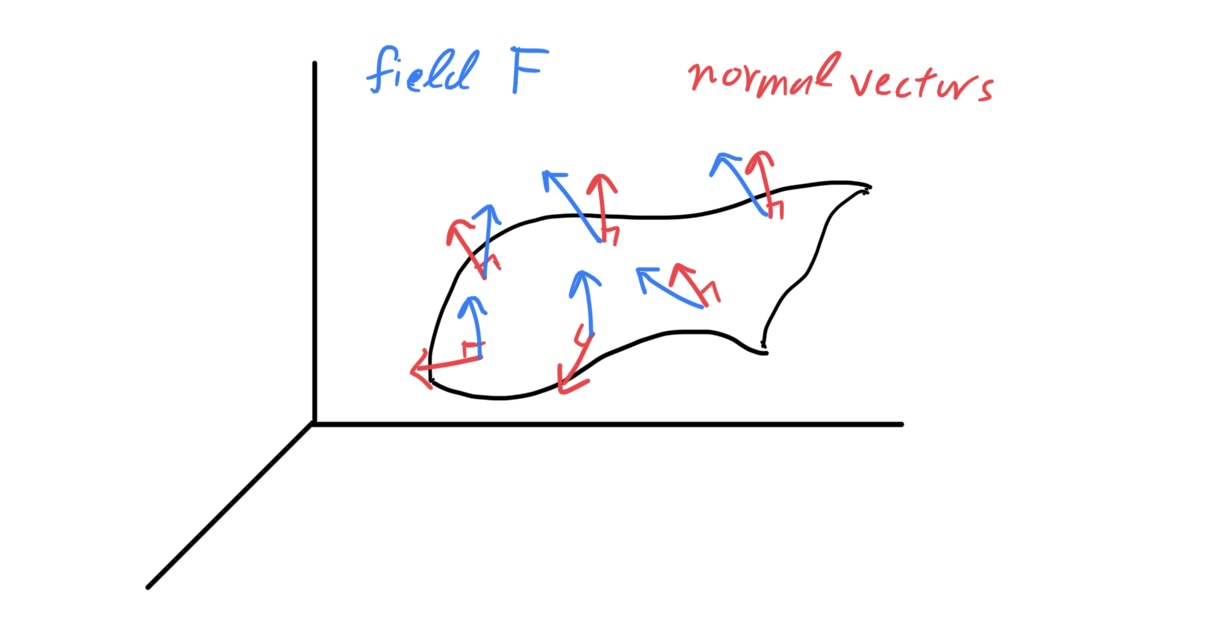
\includegraphics[scale=0.3]{img/Vector_Surface_Integral.jpg}
  \end{center}
  It can be calculated with the following formulas by converting it into a scalar surface integral where the scalar field is the value of the dot product of the vector field with the normal vectors of the surface. 
  \begin{align*}
      \iint_{S} F \cdot d S & = \iint_S (F \cdot n) \; dS \\
      & = \iint_D \Bigg( F\big( \varphi(u, v)\big) \cdot \frac{\frac{\partial \varphi}{\partial u} \times \frac{\partial \varphi}{\partial v}}{\Big|\Big|\frac{\partial \varphi}{\partial u} \times \frac{\partial \varphi}{\partial v} \Big|\Big|} \Bigg) \, \bigg|\bigg|\frac{\partial \varphi}{\partial u} \times \frac{\partial \varphi}{\partial v}\bigg|\bigg|\; du\,dv \\
      & = \iint_D F\big(\varphi(u, v)\big) \cdot \bigg( \frac{\partial \varphi}{\partial u} \times \frac{\partial \varphi}{\partial v}\bigg) \; du\,dv
  \end{align*}
  \end{definition}

  Since we are now talking about vector fields, the orientation of the paramaterization is now significant. Visually, if the orientation of the surface $S$ generally aligns with the vector field $F$, then the integral will be positive (since two vectors $\alpha, \beta$ generally pointing in the same direction implies that $\alpha \cdot \beta > 0$). The orientation of the paramaterization, which is dependent on $\frac{\partial \varphi}{\partial u} \times \frac{\partial \varphi}{\partial v}$, determines the direction of the normal vector $n$ (since it is defined to be $(\frac{\partial \varphi}{\partial u} \times \frac{\partial \varphi}{\partial v}) / \big|\big|\frac{\partial \varphi}{\partial u} \times \frac{\partial \varphi}{\partial v}\big|\big|$. Therefore, changing the orientation of $\varphi$ will reverse the direction of $n$, which will then reverse the sign of the integral since $n$ now points in the opposite direction of the vector field $F$ than it previously did (by reversing the sign of the dot products). This is formalized in the theorem below. 

  \begin{theorem}[Invariance of Surface Paramaterizations on Vector Surface Integrals]
  Let $S$ be an oriented surface and let $\varphi_1$ and $\varphi_2$ be two regular paramaterizations with $F$ a continuous vector field defined on $S$. Then, assuming $\varphi_1$ is orientation preserving, 
  \begin{align*}
      \varphi_2 \text{ is orientation preserving } & \implies \iint_{\varphi_1} F \cdot d S = \iint_{\varphi_2} F \cdot d S \\
      \varphi_2 \text{ is orientation reversing } & \implies - \iint_{\varphi_1} F \cdot d S = \iint_{\varphi_2} F \cdot d S 
  \end{align*}
  \end{theorem}

  \subsubsection{Surface Integrals over Graphs}
  Given that we have the graph of a function $g: \mathbb{R}^2 \longrightarrow \mathbb{R}$ rather than a general surface, we can paramaterize it simply as
  \[\varphi(u, v) \equiv \big(u, v, g(u, v) \big)\]
  \begin{center}
      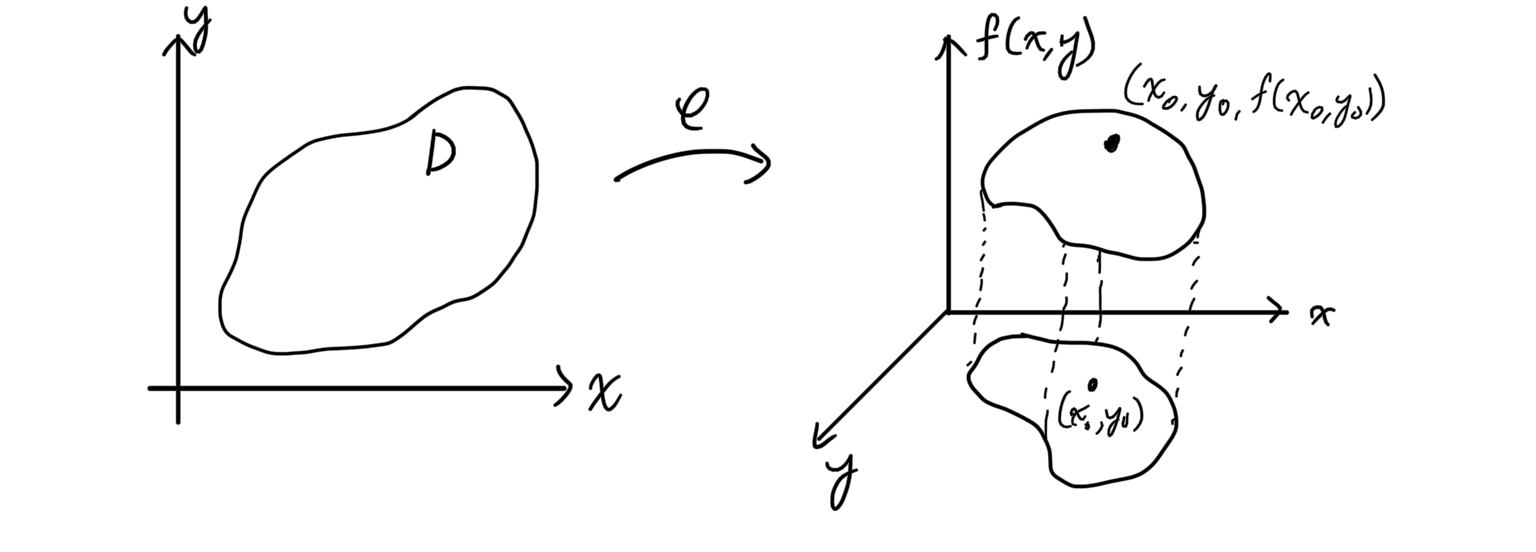
\includegraphics[scale=0.25]{img/Paramaterize_Surfaces_as_Graphs.PNG}
  \end{center}
  This means that 
  \[\frac{\partial \varphi}{\partial u} \times \frac{\partial \varphi}{\partial v} = 
  \begin{pmatrix}
  -\frac{\partial g}{\partial u} \\ -\frac{\partial g}{\partial v} \\ 1
  \end{pmatrix} \implies \bigg|\bigg|\frac{\partial \varphi}{\partial u} \times \frac{\partial \varphi}{\partial v} \bigg|\bigg| = \sqrt{1 + \Big(\frac{\partial g}{\partial u}\Big)^2 + \Big( \frac{\partial g}{\partial v}\Big)^2}\]
  So we can simplify the equation for the surface area $S$ of the graph of $g$ over the region $D$ in the $x y$-plane, as 
  \begin{align*}
      A(S) & = \iint_S \; d S = \iint_D \bigg|\bigg|\frac{\partial \varphi}{\partial u} \times \frac{\partial \varphi}{\partial v} \bigg|\bigg| \; d A \\
      & = \iint_D \sqrt{1 + \Big(\frac{\partial g}{\partial u}\Big)^2 + \Big( \frac{\partial g}{\partial v}\Big)^2} \; d u \, d v
  \end{align*}
  With the same $g$, we can find the weighed surface area of $S$ over the scalar function $f: \mathbb{R}^3 \longrightarrow \mathbb{R}$ with the formula
  \[\iint_S f \; d S = \iint_D f\big(u, v, g(u, v)\big) \sqrt{1 + \Big(\frac{\partial g}{\partial u}\Big)^2 + \Big( \frac{\partial g}{\partial v}\Big)^2} \; d u \, d v\]
  Finally, with the same graph $g$, the surface integral over the vector field $F$ is
  \begin{align*}
      \iint_S F \cdot d S & = \iint_D F\big(\varphi(u, v)\big) \cdot \bigg( \frac{\partial \varphi}{\partial u} \times \frac{\partial \varphi}{\partial v}\bigg) \; d u \, d v \\
      & = \iint_D \bigg( F_1(u, v) \Big(- \frac{\partial g}{\partial u}\Big) + F_2 (u, v) \Big( - \frac{\partial g}{\partial v} \Big) + F_3 (u, v) \bigg) \; d u \, d v
  \end{align*}

\subsection{Integral Theorems}

  Recall the differential notation for writing line integrals. For 2 and 3 dimensions, it is written as
  \begin{align*}
      & \int_C F \cdot d s = \int_C F \cdot (d x, d y) = \int_C F_1 \, d x + F_2 \, d y \\
      & \int_C F \cdot d s = \int_C F \cdot (d x, d y, d z) = \int_C F_1 \, d x + F_2 \, d y + F_3 \, d z 
  \end{align*}
  \subsubsection{Green's Theorem}
  Green's Theorem gives the relationship between a line integral around a simple closed curve $C$ and a double integral over the plane region $D$ bounded by $C$. 

  \begin{theorem}[Green's Theorem in $\mathbb{R}^2$]
  Let there be a 2-dimensional $C^1$ vector field $F$ on $\mathbb{R}^2$ defined on a simple oriented closed piecewise-smooth curve $C$ and its bounded region $D \subset \mathbb{R}^2$ (that is, $C = \partial D$). Let the orientation of the path of $C$ be such that it is traveling \textit{counterclockwise}, i.e. a point traveling through $C$ would see the region $D$ to its \textit{left}, denoted as $C^+$ and the clockwise orientation as $C^-$.  Then, 
  \[\oint_{C^+} F_1 \, d x + F_2 \, d y = \iint_D \bigg( \frac{\partial F_2}{\partial x} - \frac{\partial F_1}{\partial y} \bigg) \; d x \, d y\]
  By reversing the orientation, it is clear that we have
  \[\oint_{C^-} F_1 \, d x + F_2 \, d y = - \iint_D \bigg( \frac{\partial F_2}{\partial x} - \frac{\partial F_1}{\partial y} \bigg) \; d x \, d y\]
  Note that this theorem is expressed in terms of the components of the vector field $F$. 
  \begin{center}
  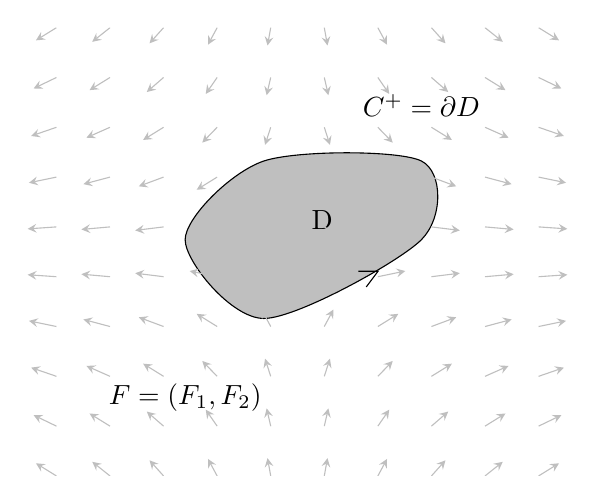
\begin{tikzpicture}
      \draw[fill=lightgray] plot [smooth cycle] coordinates {(2,3) (3,4) (5,4) (5,3) (3,2)};
      \node [above left] at (4,3) {D};
      \begin{axis}[view={0}{90}, hide axis, zmin=-1, zmax=1]
      \addplot3 [lightgray,-stealth,samples=10,
          quiver={
              u={3*x/pow(x^2 + y^2,1/2)},
              v={-2*y/pow(x^2 + y^2,1/2)},
              scale arrows=0.2,
          },] {0};
      \end{axis}
      \node at (2,1) {$F = (F_1, F_2)$};
      \node at (5,4.7) {$C^+ = \partial D$};
      \draw (4.3,2.4)--(4.45,2.6)--(4.2,2.6);
  \end{tikzpicture}
  \end{center}
  \end{theorem}

  Green's theorem has many applications in physics. For example, in order to solve two-dimensional flow integrals measuring the sum of fluid outflowing from a volume, Green's theorem allows us to calculate the total outflow summed about an enclosing area . 

  \begin{corollary}
  Let $D$ be a region for which Green's theorem applies with positively oriented boundary $\partial D$. Then, the area of $D$ can be computed with the formula
  \[A(D) = \frac{1}{2} \oint_{\partial D} x \, d y - y \, d x\]
  \end{corollary}

  Green's theorem can be used to determine the area of centroid of plane figures solely by integrating over the perimeter. 

  \subsubsection{Stokes' Theorem}
  Green's theorem relates line integrals to double integrals. Stokes' theorem generalizes Green's theorem by relating line integrals to surface integrals of 2-dimensional surfaces embedded in $\mathbb{R}^3$. 

  \begin{theorem}[Stokes' Theorem]
  Let $S$ be an oriented regular surface defined by paramaterization $\varphi: D \subset \mathbb{R}^2 \longrightarrow \mathbb{R}^3$, and let the image of the boundary $\partial D$ under $\varphi$ be the boundary $\partial S$ of $S$. We can interpret $\partial S$ as a path mapping from $\mathbb{R} \longrightarrow S \subset \mathbb{R}^3$. 
  \begin{center}
    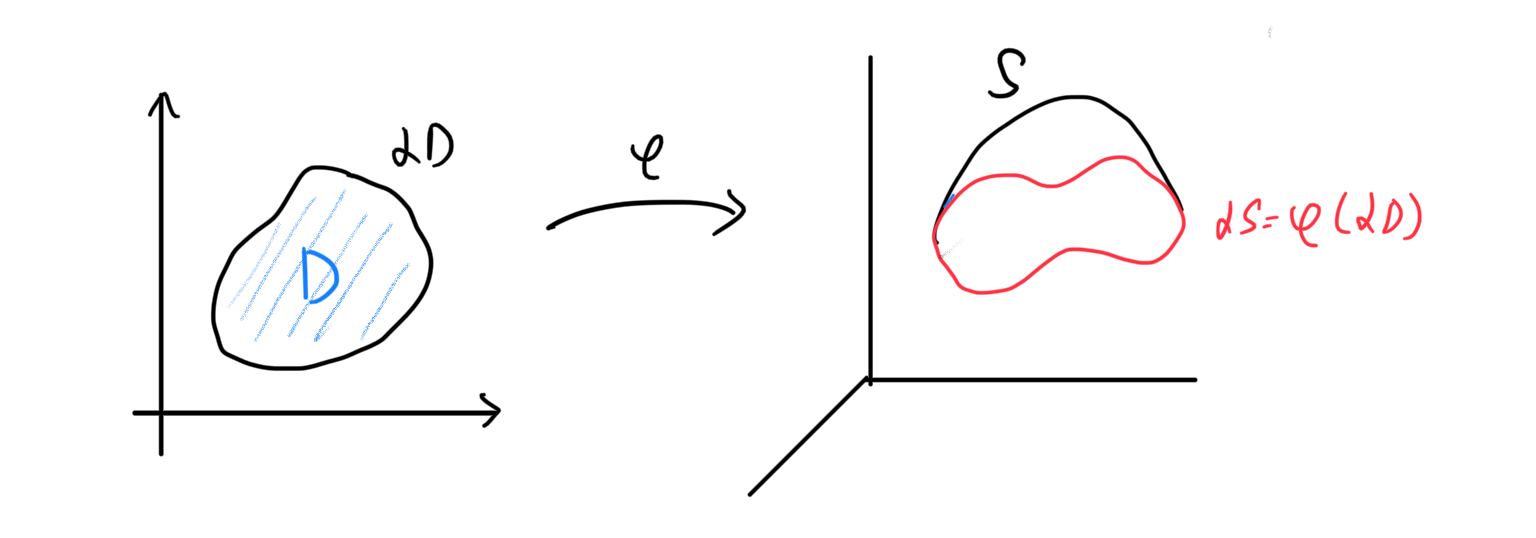
\includegraphics[scale=0.27]{img/Boundary_Mapping.PNG}
  \end{center}
  The orientation unit vector $n$ of $S$ induces the positive orientation of $\partial S$, denoted $\partial S^+$. Visually, if you are walking along the curve with your head is pointing in the same direction as the unit normal vectors while the surface is on the left then you are walking in the positive direction on $\partial S$. 
  \begin{center}
      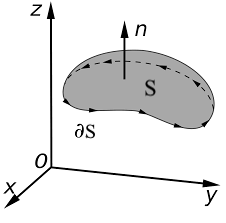
\includegraphics[scale=0.8]{img/Stokes_Theorem_Orientation.png}
  \end{center}
  Given that $F$ is a $C^1$ vector field defined on $S$, then
  \[\iint_S \curl{F} \cdot dS = \iint_S \big( \nabla \times F \big) \cdot d S = \oint_{\partial S^+} F \cdot d s\]
  If $S$ has no boundary, that is, if the image of $p^\prime = \partial S$ is not a simple closed curve, then the integral is $0$. 
  \end{theorem}

  The above theorem implies that the vector surface integral of a surface without a boundary (i.e. a closed graph, such as a sphere) is always $0$ along the curl of any $C^1$ field. Geometrically, this means that given a closed solid $S$ with field $\nabla \times F$, the rate of flow of the vector field into $S$ is equal to the flow out of $S$. 

  \subsubsection{Gauss' Theorem}
  The divergence theorem relates the flux of a vector field through a closed surface to the divergence of the field in the volume enclosed. 

  \begin{theorem}[Gauss' Divergence Theorem]
  Let $V$ be a subset of $\mathbb{R}^3$. Denote by $\partial V$ the oriented closed surface that bounds $V$ (with outward pointing normal orientation vectors), and let $F$ be a $C^1$ vector field defined on a neighborhood of $V$. Then, 
  \[\iiint_V \Div{F} \; d V = \iiint_V (\nabla \cdot F) \; d V = \oiint_{\partial V} F \cdot d S = \oiint_{\partial V} (F \cdot n) \; dS\]
  where the two left-most integrals are volume integrals, and the two right-most integrals are surface integrals. Intuitively, this makes sense; the volume integrals represent the total of the sources in volume $V$, and the right hand side represents the total flow across the boundary $\partial V$. 
  \begin{center}
      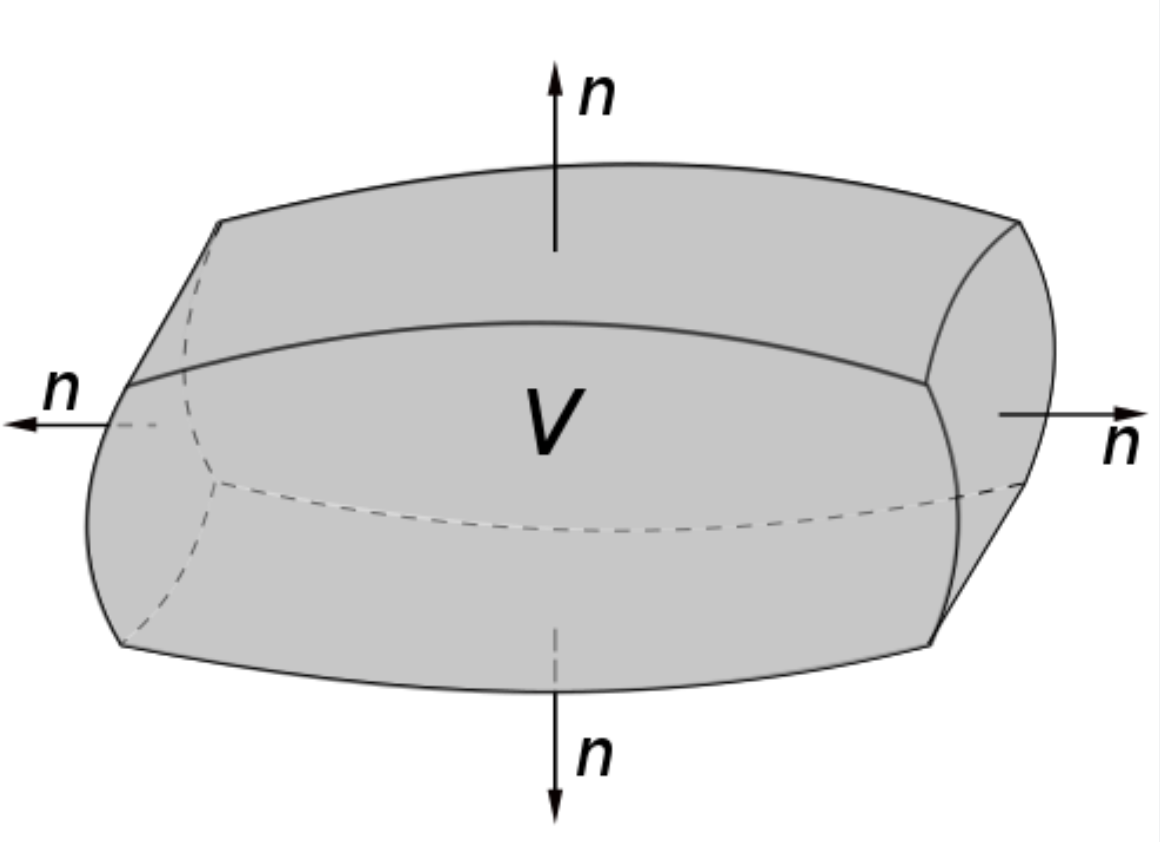
\includegraphics[scale=0.35]{img/Gauss_Theorem_Volume.png}
  \end{center}
  \end{theorem}
